%%%%%%%%%%%%%%%%%%%%%%%%%%%%%%%%%%%%%%%
% Wenneker Resume/CV
% LaTeX Template
% Version 1.1 (19/6/2016)
%
% This template has been downloaded from:
% http://www.LaTeXTemplates.com
%
% Original author:
% Frits Wenneker (http://www.howtotex.com) with extensive modifications by 
% Vel (vel@LaTeXTemplates.com)
%
% License:
% CC BY-NC-SA 3.0 (http://creativecommons.org/licenses/by-nc-sa/3.0/
%
%%%%%%%%%%%%%%%%%%%%%%%%%%%%%%%%%%%%%%

%----------------------------------------------------------------------------------------
%	PACKAGES AND OTHER DOCUMENT CONFIGURATIONS
%----------------------------------------------------------------------------------------

\documentclass[a4paper,12pt]{memoir} % Font and paper size
\usepackage[pdfstartview=FitH,
bookmarks=true,
bookmarksnumbered=true,
bookmarksopen=false,
colorlinks, %注释掉此项则交叉引用为彩色边框(将colorlinks和pdfborder同时注释掉)
%pdfborder=001,   %注释掉此项则交叉引用为彩色边框
linkcolor=cyan,
anchorcolor=cyan,
citecolor=cyan]{hyperref}

%%%%%%%%%%%%%%%%%%%%%%%%%%%%%%%%%%%%%%%%%
% Wenneker Resume/CV
% Structure Specification File
% Version 1.1 (19/6/2016)
%
% This file has been downloaded from:
% http://www.LaTeXTemplates.com
%
% Original author:
% Frits Wenneker (http://www.howtotex.com) with extensive modifications by 
% Vel (vel@latextemplates.com)
%
% License:
% CC BY-NC-SA 3.0 (http://creativecommons.org/licenses/by-nc-sa/3.0/)
%
%%%%%%%%%%%%%%%%%%%%%%%%%%%%%%%%%%%%%%%%%

%----------------------------------------------------------------------------------------
%	PACKAGES AND OTHER DOCUMENT CONFIGURATIONS
%----------------------------------------------------------------------------------------

\usepackage{XCharter} % Use the Bitstream Charter font
\usepackage[utf8]{inputenc} % Required for inputting international characters
\usepackage[T1]{fontenc} % Output font encoding for international characters

\usepackage[top=1.5cm,left=0cm,right=0.2cm,bottom=1.5cm]{geometry} % Modify margins

\usepackage{graphicx} % Required for figures

\usepackage{flowfram} % Required for the multi-column layout

\usepackage{url} % URLs

\usepackage[usenames,dvipsnames]{xcolor} % Required for custom colours

\usepackage{tikz} % Required for the horizontal rule

\usepackage{enumitem} % Required for modifying lists
\setlist{noitemsep,nolistsep} % Remove spacing within and around lists

\setlength{\columnsep}{\baselineskip} % Set the spacing between columns

% Define the left frame (sidebar)
\newflowframe{0.3\textwidth}{\textheight}{0pt}{0pt}[left]
\newlength{\LeftMainSep}
\setlength{\LeftMainSep}{0.3\textwidth}
\addtolength{\LeftMainSep}{1\columnsep}
 
% Small static frame for the vertical line
\newstaticframe{1.5pt}{\textheight}{\LeftMainSep}{0pt}
 
% Content of the static frame with the vertical line
\begin{staticcontents}{1}
\hfill
\tikz{\draw[loosely dotted,color=RoyalBlue,line width=1.5pt,yshift=0](0,0) -- (0,\textheight);}
\hfill\mbox{}
\end{staticcontents}
 
% Define the right frame (main body)
\addtolength{\LeftMainSep}{1.5pt}
\addtolength{\LeftMainSep}{1\columnsep}
\newflowframe{0.6\textwidth}{\textheight}{\LeftMainSep}{0pt}[main01]

\pagestyle{empty} % Disable all page numbering

\setlength{\parindent}{0pt} % Stop paragraph indentation

%----------------------------------------------------------------------------------------
%	NEW COMMANDS
%----------------------------------------------------------------------------------------

\newcommand{\userinformation}[1]{\renewcommand{\userinformation}{#1}} % Define a new command for the CV user's information that goes into the left column

\newcommand{\cvheading}[1]{{\Huge\bfseries\color{RoyalBlue} #1} \par\vspace{.6\baselineskip}} % New command for the CV heading
\newcommand{\cvsubheading}[1]{{\Large\bfseries #1} \bigbreak} % New command for the CV subheading

\newcommand{\Sep}{\vspace{1em}} % New command for the spacing between headings
\newcommand{\SmallSep}{\vspace{0.5em}} % New command for the spacing within headings

\newcommand{\aboutme}[2]{ % New command for the about me section
\textbf{\color{RoyalBlue} #1}~~#2\par\Sep
}
	
\newcommand{\CVSection}[1]{ % New command for the headings within sections
{\Large\textbf{#1}}\par
\SmallSep % Used for spacing
}

\newcommand{\CVItem}[2]{ % New command for the item descriptions
\textbf{\color{RoyalBlue} #1}\par
#2
\SmallSep % Used for spacing
}

\newcommand{\bluebullet}{\textcolor{RoyalBlue}{$\circ$}~~} % New command for the blue bullets
 % Include the file specifying document layout and packages

%----------------------------------------------------------------------------------------
%	NAME AND CONTACT INFORMATION 
%----------------------------------------------------------------------------------------

\userinformation{ % Set the content that goes into the sidebar of each page
\begin{flushright}
% Comment out this figure block if you don't want a photo
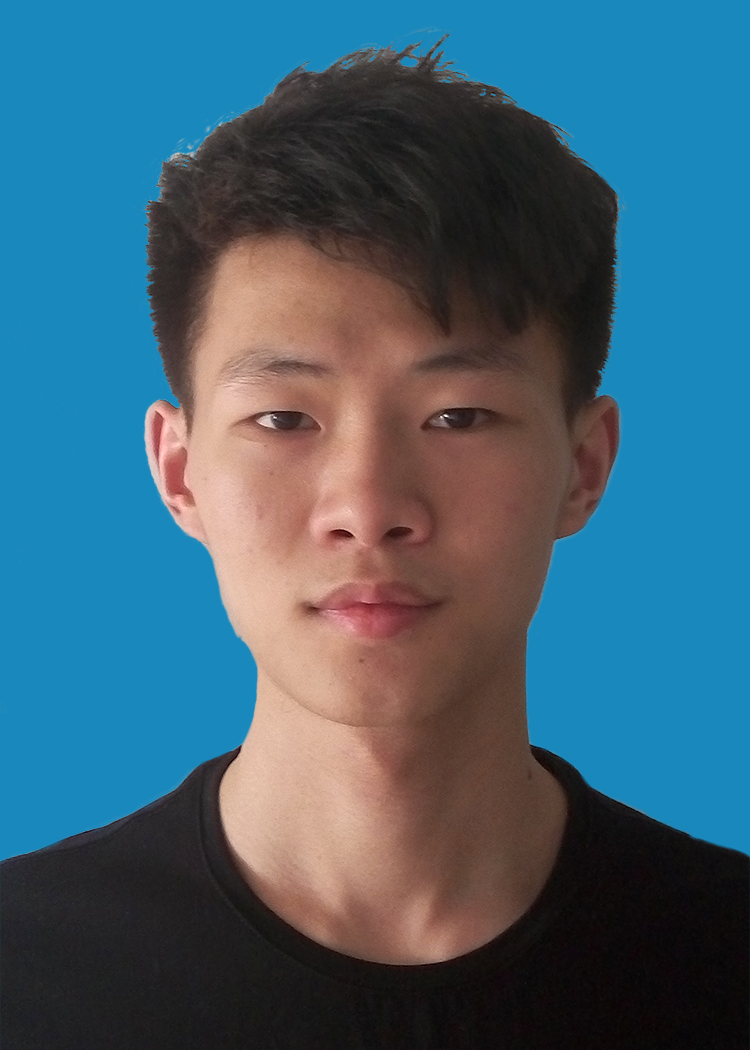
\includegraphics[width=0.6\columnwidth]{photo.jpg}\\[\baselineskip] % Your photo
\small % Smaller font size
\textbf{Xu Wei} \\ % Your name
(+86) 155--7434--9704 \\ % Your phone number
\url{xuwei3893@csu.edu.cn} \\ % Your email address
\url{https://github.com/CSQ223} \\ % Your URL
\Sep % Some whitespace
\textbf{Address} \\
Central South University \\ % Address 1
Changsha, Hunan, China \\ % Address 2
410075 \\ % Address 3
\vfill % Whitespace under this block to push it up under the photo
\end{flushright}
}

%----------------------------------------------------------------------------------------

\begin{document}

\userinformation % Print your information in the left column

\framebreak % End of the first column

%----------------------------------------------------------------------------------------
%	HEADING
%----------------------------------------------------------------------------------------

\cvheading{Xu Wei} % Large heading - your name

\cvsubheading{Logistics Engineering} % Subheading - your occupation/specialization
\CVItem{Research Interests}{Vehicle Routing Problem\\Metaheuristics\\Exact Solution Method}

%----------------------------------------------------------------------------------------
%	ABOUT ME
%----------------------------------------------------------------------------------------

%\aboutme{About Me}{Lorem ipsum dolor sit amet, consectetur adipiscing elit. Vivamus vel bibendum metus. Proin rutrum pharetra molestie. Cras sollicitudin nulla nec leo lobortis in tristique purus pretium. Ut eu felis nulla. Pellentesque condimentum justo ut ligula feugiat nec facilisis tellus ultricies. Nullam sit amet dictum ipsum. Sed lacus neque, hendrerit eu rhoncus nec, pellentesque vitae sem.}

\CVItem{}{}

%----------------------------------------------------------------------------------------
%	EDUCATION
%----------------------------------------------------------------------------------------

\CVSection{Education}

%------------------------------------------------

\CVItem{\textit{09.2018 -- Present,} Central South University} {MEng in Logistics Engineering\\
	\begin{tabular}{ @{} >{\bfseries}l @{\hspace{1ex}} l }
		Main Cources: & Advanced Engineering Methematics\\
		& Advanced Operation Research \\
		& Traffic Network Equilibrium Theory
	\end{tabular}}

%------------------------------------------------

\CVItem{\textit{09.2014 -- 07.2018,} Central South University of Forest and Technology}{B.E. in Logistics Engineering \hfill Grade: $87.21\%$}

%------------------------------------------------

\Sep % Extra whitespace after the end of a major section

%----------------------------------------------------------------------------------------
%	AWARDS
%----------------------------------------------------------------------------------------
\CVSection{Awards}
%------------------------------------------------
\CVItem{2016, \textit{The Second Prize of CUMCM}}{Contemporary Undergraduate Mathematical Contest in Modeling}

\CVItem{2018, \textit{The Award of Outstanding Graduates }}{Central South University of Forest and Technology}
%------------------------------------------------
\Sep % Extra whitespace after the end of a major section

%----------------------------------------------------------------------------------------
%	SKILLS
%----------------------------------------------------------------------------------------

\CVSection{Tech Skills}

%------------------------------------------------

\CVItem{Programming Languages} {
	\begin{tabular}{ @{} >{\bfseries}l @{\hspace{1ex}} l }
		C++ & VRP, GUI with Qt Framework\\
		Python & Spider, sklearn\\
		Java & Cplex API Language\\
		MATLAB & Scientific Computing
\end{tabular}}

%------------------------------------------------
\CVItem{Database} {
	\begin{tabular}{ @{} >{\bfseries}l @{\hspace{6ex}} >{\bfseries}l @{\hspace{6ex}} >{\bfseries}l }
		MYSQL & SQLIte & SQL Server
\end{tabular}}

%------------------------------------------------
\CVItem{Tools} {
	\begin{tabular}{ @{} >{\bfseries}l @{\hspace{6ex}} >{\bfseries}l @{\hspace{6ex}} >{\bfseries}l }
		\LaTeX & Illustrator & Photoshop
\end{tabular}}
\Sep % Extra whitespace after the end of a major section


%----------------------------------------------------------------------------------------
%	EXPERIENCE
%----------------------------------------------------------------------------------------

\CVSection{Personal Work}

%------------------------------------------------

\CVItem{\textit{03.2018 -- 05.2018}, Undergraduate Graduation Design}{
\emph{Design and Implementation of Regional Bicycle Dispatching System for Shared Bicycles}
\begin{itemize}
	\item establishes a mathematical model for Vehicle Routing Problem;
	\item designs a Genetic Algorithm for the model;
	\item codes in C++ language and implements GUI with Qt Framework;
	\item stores and queries data with MYSQL.
\end{itemize}
}
%------------------------------------------------

\Sep % Extra whitespace after the end of a major section



%----------------------------------------------------------------------------------------
%	NEW PAGE DELIMITER
%	Place this block wherever you would like the content of your CV to go onto the next page
%----------------------------------------------------------------------------------------

%\clearpage % Start a new page

%\userinformation % Print your information in the left column

%\framebreak % End of the first column




\end{document}
